\scanpage{85}
% archive sheet number: 84
% Three large diagonal cancellation strokes cross the typescript.
\deleted{\uline{Remarques} \raisebox{2ex}{\inserted{\handwritten{4}}} a) On se gardera de croire que lorsque $A$ est un anneau n\unsure{\rlap{e}o|o}et\rlap{é}h\rlap{h}érien, $B$ une $A$-algèbre plate de type fini, $(J_i)_{i\quad I}$ une famille d'idéaux de $A$ dont l'intersection est nulle, alors l'intersection des $J_iB$ soit nulle. (On a déjà signalé l'exemple d'un anneau de valuation discrète $A$, muni des \mbox{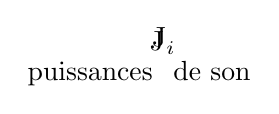
\begin{tikzpicture}[baseline=(left.base)]
\node[inner sep=0] (left) {puissances};
\node[anchor=base west,inner sep=0,xshift=.25cm] at (left.base east) {de son};
\node[anchor=south west,inner sep=0,xshift=-.05cm,yshift=.08cm] at (left.north east) {\inserted{$\text{\rlap{J}\raisebox{.3ex}{\kern.08em J}}_i$}};
\end{tikzpicture}} idéal maximal, et $B$ étant le corps des fractions). \deleted{Le fait} En effet, l'hypothèse que $\quad J_i=0$ n'implique nullement que $\quad J_i=0$ !}

\deleted{b) Soit $X$ un préschéma sur un corps $k$, et soit $u_i\colon Z_i\quad X$ une famille schématiquement dominante. Nous ignorons si pour tout changement de base $S\quad\operatorname{Spec}(k)$, la famille des $u_{i\,S}\colon Z_{i\,S}\quad X_S$ est sch. \mbox{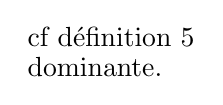
\begin{tikzpicture}[baseline=(base.base)]
\node[inner sep=0] (base) {dominante.};
\node[anchor=south west,inner sep=0,yshift=.12cm] at (base.north west) {\inserted{cf définition 5}};
\end{tikzpicture}} On peut \deleted{se ram} montrer (par des arguments du type de ceux utilisés ci-dessous) qu'il suffit pour cela que cette propriété soit satisfaite chaque fois que $S$ est le spectre d'un corps $k'$ extension finie séparable de $k$. D'autre part, nous verrons ci-dessous que la réponse est affirmative lorsque $X$ est localement noethérien.}

\deleted{\uline{Définition} 5. Sous les notations de 1., supposons que $X$ soit un $S$-préschéma. On dit que $(u_i)$ est \deleted{relativement} schématiquement dominante relativement à $S$ \deleted{(ou que la famille des sous-préschémas $Z_i$, s'il s'agit de tels, est sch dense dans $X$ rel à $S$)} si pour tout $S'\quad S$, la famille des $u_{i\,S'}\colon Z_{i\,S'}\quad X_{S'}$ est sch dominante \deleted{(resp ou que la famille} Quand les $Z_i$ sont des sous-préschémas de $X$ \ldots, on dit aussi que la famille \deleted{des} $\unsure{(Z_i)|\{Z_i)}$ est sch dense dans $X$ rel à $S$.}

\deleted{NB C'est une notion locale sur $X$ et sur $S$.}

\deleted{\uline{Lemme} 6\quad Avec les notations précédentes, supposons $X$ et les $Z_i$ plats sur $S$, soit $S_o$ un sous-préschéma de $S$ défini par un Idéal Nilpotent. Si la famille des $u_{i\,S_o}$ est sch dominante, il en est de même de la famille des $u_i$. On peut resper avec ``rel à $S$''.}

\deleted{La deuxième assertion résulte trivialement de la première et des définitions. Pour la première, cf SGAD IX. 4.2.}
